% $Id: evaluation.tex 
% !TEX root = ../main.tex

\section{Empirical Study}
\label{sec:evaluation}

This section presents the empirical study for \flik. The purpose of the empirical study assessing the 
user experience and usefulness of \flik, when used to identify and locate bugs in  \ac{RL} programs. 
In particular, the participants were provided with three different \ac{RL} programs that implement three 
\ac{RL} problems. The problems were chosen according to their familiarity and an increasing 
environment complexity. 
\begin{enumerate*}[label=(\arabic*)]
\item GridWorld, is a standard benchmark for \ac{RL} based on episodic learning.
\item Rooms, is common \ac{RL} problem used as an example of the complexity of environments and 
the possibility por agents to abstract their knowledge in hierarchical learning~\cite{pateria21} 
structures. \item Finally, Driving assistant is a more recent \ac{RL} environment, uncommon to most 
developers, used to learn different tasks for autonomous driving in a continuous environment. 
\end{enumerate*}

A fault was manually injected in each program, and the task assigned to the participants was to improve the functional quality of the three programs. Note that the injected bugs did not lead the program to exceptions or crashes, i.e., each program ran and there was no evident buggy behavior. The injected bugs made the programs to generate outputs that do not match the expected outputs. Concerning the participants, master students from the Reinforcement Learning course at Universidad de los Andes were recruited.  The participants were provided with a evaluation  \fref{sec:eval-guide}, that describes the purpose of the tool, the task and steps, instructions on how to run and 
use the tool, documentation of the tool, and an small example. The real-world problems implemented for the study are described in the following:

%%%%
\paragraph{\textbf{GridWorld.}}
This environment consists of a $n \times n$ ($10\times 10$ in our example) 
rectangular  board/grid, in which each tile $(i,j)$ represents a specific state of the board. Tiles in the board may be  walls, which agents cannot cross. Additionally, there are special exit  tiles that give a positive or negative reward to agents, as shown in \fref{fig:gridworld}. All tile types are unknown to the agent that moves from a given starting point in the board, searching for the goal state (\ie exit states with positive reward of $1$). The agent moves from state to state, avoiding  obstacles and incorrect exit states (which give a reward of $-1$ when used to exit). 

The program has a bug for the $\epsilon$ parameter, presenting an error in the probability which defines which action is taken next. This introduces a wrong behavior for the \ac{RL} 
agent because $\epsilon$ will be so small that only in the first iteration the action will be taken randomly and in the follow iterations the probability will be so small to take another action that the agent will not explore other action policies. This is an undesired behavior specially for training purposes as an agent should have a large probability to choose other actions and explore the grid. The idea in this task is that the study participants use \flik to navigate through the code and find out why the agent is not learning properly. And eventually, the participants should come out with the solution of increasing the value of $\epsilon$. 

\begin{figure}[hptb]
  \centering
  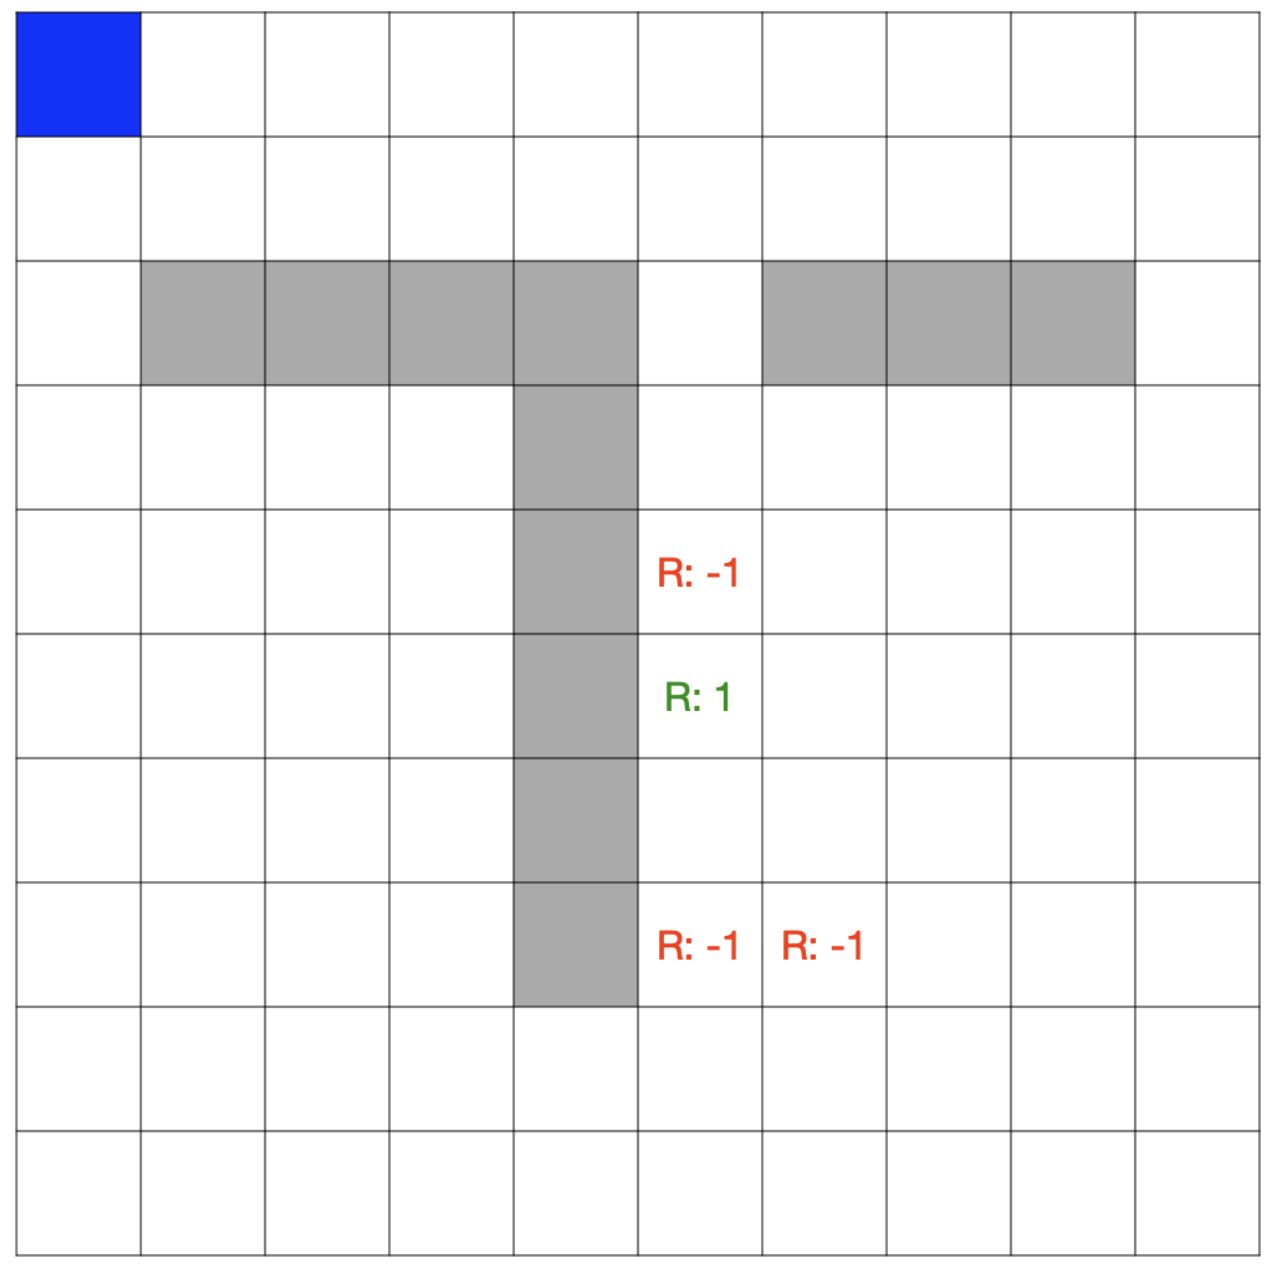
\includegraphics[width=0.5\columnwidth]{figures/gridworld.png}
  \caption{10x10 gridworld environment example}
  \label{fig:gridworld}
\end{figure}

%%%%
\paragraph{\textbf{Rooms.}} 
The four rooms maze environment consists of a $13\times 13$ board/grid divided in $4$ sections 
(\ie rooms), with walls between them, and a door opening to go from one room to another, as shown 
in \fref{fig:rooms}. The agent's objective in this environment is to exit through the upper-left room 
(the green square) in the fewest possible steps. Reaching the exit state gives a reward of $1$, and no 
other action give a reward to the agent. In each episode the agent starts from any valid position in the 
grid, \eg the yellow square in the bottom-right room in the figure. 

\begin{figure}[hptb]
  \centering
  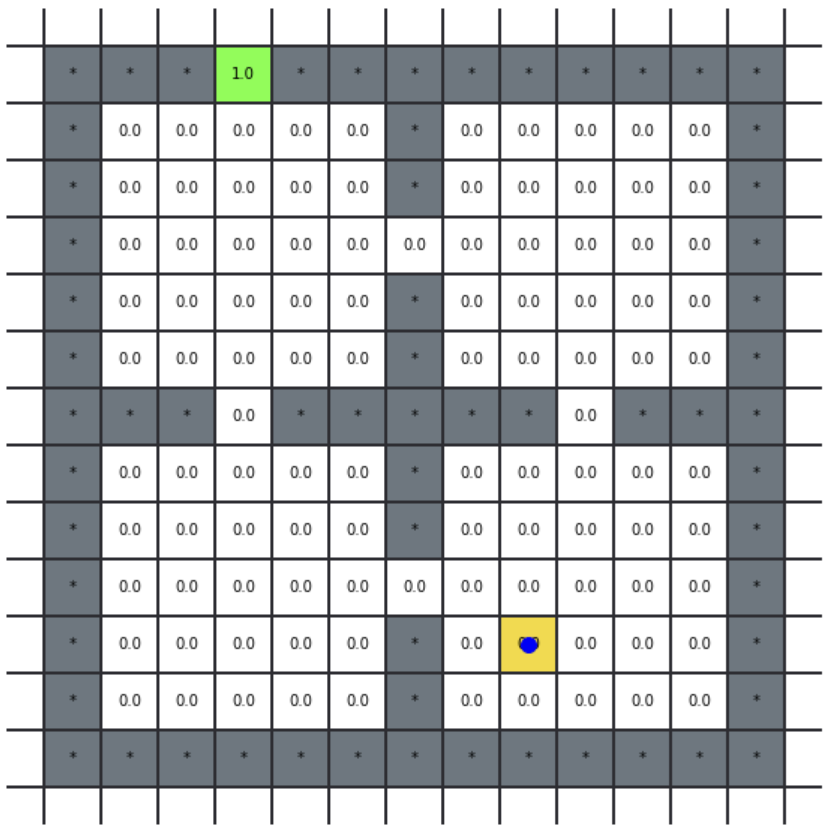
\includegraphics[width=0.5\columnwidth]{figures/rooms.png}
  \caption{Rooms environment example with associated rewards in each state}
  \label{fig:rooms}
\end{figure}

In the program, we introduced a bug in the learning rate $\alpha$, on the Q-learning equation, thus,  the original values for the learning rate alpha are exchanged like:

\begin{itemize}
\item Original equation:
$
Q(s, a) \leftarrow (1-\alpha) Q(s, a) + \alpha \left( r + \gamma \max_{a'} Q(s', a') \right)
$

\item Erroneous equation to debug:
$
Q(s, a) \leftarrow  \alpha Q(s, a) + (1-\alpha) \left( r + \gamma \max_{a'} Q(s', a') \right)
$
\end{itemize}

In the original equation,  $(1-\alpha) Q(s, a)$ is the current value and $\gamma \max_{a'} Q(s', a')$ 
the maximum reward that can be obtained from state $s'$. This means that if the learning rate is very 
small the current value will keep almost the same, turning a little bit towards the reward and the 
maximum value given the action; this will make that the agent learn short steps towards the 
optimal policy. In the Q-learning formula, the learning rate $\alpha$ defines how much the old estimate $Q(s,a)$ 
is revised based on the new information. It ensures that over time, the algorithm balances past 
knowledge with current learning, gradually incorporating new information while retaining important 
aspects of previous learning. Changing the equation in this way will disrupt this balance. Specifically,
$(1-\alpha)$ scales the difference between the new estimate and the old estimate. This makes the new information less influential as $\alpha$ gets larger, while the old value gets re-scaled by $\alpha$,  which does not align with the expected behavior of a Q-learning update. The idea in this task is that the participants use \flik to navigate through the code and find out the reason why the agent is not learning properly, afterwards we expected the participant to figure out a solution adjusting the proper value to update the Q-Learning equation.

%\subsection{Exercise 3: Driving Assistant}
%\label{sec:cars-eval}
\paragraph{\textbf{Cars (Driving Assistant).}} In this case the agent must learn to drive, on the correct lane, at the allowed speed, taking over slow traffic, and not crashing. The possible actions for the agent are: straight, slow\_down, speed\_up, steer\_left, steer\_right. Figure \ref{fig:cars-code-example} depicts the visual interface of this environment.

\begin{figure}[h]
    \centering
    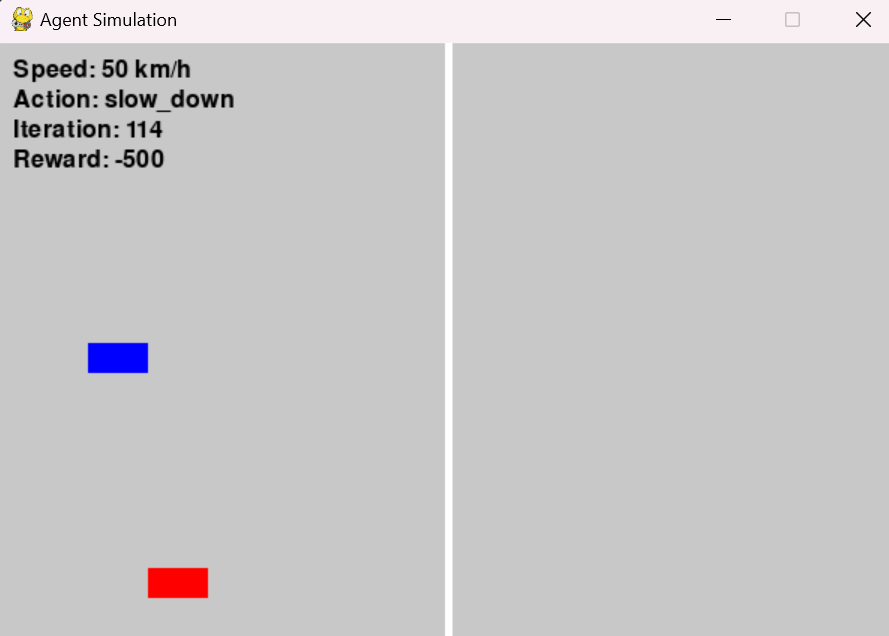
\includegraphics[width=0.5\textwidth]{figures/cars_example.png}
    \caption{Cars code example}
    \label{fig:cars-code-example}
\end{figure}

This is the largest task for the participants to analyze with \flik. % and see why the agent was not learningcorrectly, with respect to the expected. 
The bug introduced in this application is in the reward function, not motivating the agent to drive at the speed limit. The policy learned by the agent emerges as stopping or go very slow, which is not the expected behavior. Through exploration using \flik, developers are expected to observe the behavior of the reward and update it so that the agent can learn to drive appropriately.
as expected.

%% Add way of evaluation, explanation about the survey, questions.
%\subsection{Evaluation setup}
%\label{sec:evaluation}

For the user evaluation we had a session with 27 developers (\ie graduate students). 
The developers were asked to complete the three tasks (\ie gridworld, rooms, cars) described previously. The full evaluation session used a time-slot of 1h30 split as follows 
\begin{enumerate}[label=(\arabic*)]
\item During the first 15 minutes the tool and a usage example were presented to the participants; (shown in \fref{sec:eval-guide}).
\item 50 minutes to complete the tasks; 15 minutes to finish the first task, 15 minutes to finish the second task, and  20 minutes to finish the third task. 
\item At the end of the session, the students were asked to fill an evaluation survey 
\end{enumerate}

The evaluation survey, defined as a google form, is divided in three sections: general knowledge questions, task questions, and usability.
The general knowledge questions were about the participants' experience  using Python, debuggers and  terminal. The task questions were about the bug encountered in each of the tasks, and how the the bug was fixed (if fixed). The usability  questions were regarding the participants experience with the debugger usability, and additional feedback they could provide for improving \flik. The survey was anonymized, and the questions were inspired by the 
back in time debugger for JavaScript study~\cite{leger23}, and the responses are available 
at \url{https://shorturl.at/DhN56}. 

The survey had 23 multiple choice questions with a 5-points Likert scale,  in which 5 meant completely agreed, and 1 meant completely disagreed. One of the questions was a yes or no answer, to identify if the students wanted to use the tool in the future. Finally, there were 10 open-answer questions , to dive deeper into feedback for the tool, and the tasks' complexity.


%Finally, there are two examples of the tool being used. In the first  example, the tool is used to debug a simple program, this was used to introduced to the students  the simple commands they could use like stepping (forward and backwards), modifying, or inspecting variables. In the second example, the tool is used to debug a \ac{RL} program, specially the gridworld example. The link to find this videos is: \url{https://shorturl.at/rD343} 



\endinput

